% !TEX root = ../ClassicThesis_DEIB.tex

\chapter{Background and Tools} \label{chap:backgroundAndToolsChapter}

In this chapter we are going to describe the general concepts this thesis deals with, together with the main tools we used to address the project. Since this thesis is in the frame of \ac{GRAPE} project (see Chapter \ref{chap:grapeProject}),  most of them are typical of the robotic field and, more specifically, of the agricultural robotics. This last is a part of the so-called \textit{E-agriculture}: 

%TODO http://www.fao.org/fileadmin/templates/rap/files/uploads/E-agriculture_Solutions_Forum.pdf

\section{Robot Operating System}\label{sec:robotOperatingSystem}
\ac{ROS} is the \textit{robotic middleware} we used to develop the sofware components of the system described in this thesis. We decide to use it because of its great modularity, the availability of a very large number of packages, well documented APIs and an active community. Moreover, \ac{ROS} is a very widespread system, so its power and versatility are well known in the field of software development for robotics. Citing words from its offical website\footnote{http://wiki.ros.org/ROS/Introduction},
these are \ac{ROS} main features: 
\blockquote{
\textit{It provides the services you would expect from an operating system, including hardware abstraction, low-level device control, implementation of commonly-used functionality, message-passing between processes, and package management. It also provides tools and libraries for obtaining, building, writing, and running code across multiple computers} % (TODO http://wiki.ros.org/ROS/Introduction).
} 

\ac{ROS} is actually a \textit{meta-operating system}, that is, it's not an operating system in the traditional sense (it requires to be run on top of an another operating system; currently, the only officially supported OS is Linux Ubuntu), but it provides a peer-to-peer network that processes can use to create and process data together. This network is implemented through TCP, and it's called \textit{Computation Graph}. In this section, we're going to describe \ac{ROS} with more detail, with particular emphasis on the different tecniques that nodes can use to communicate among them.
\begin{description}
\item[ROS Master] Even if the Computation Graph is a peer-to-peer network, a central process, called  \textbf{\ac{ROS} Master}, is required to exist, to provide naming and registration services to all the user processes In this. Once the processes have located each other through the services offered by the Master, they can communicate peer-to-peer without involving a central entity;

\item[nodes] The processes that are in the Computation Graph are called \textbf{nodes}, and they are the atomic units of the computational graph. The \ac{ROS} API are available in C++, Python and Lisp, but C++ is the most widely used. One of the aims of \ac{ROS} is to be modular at a fine-grained scale, so a complex task should be achieved through cooperation of several different nodes, each with quite narrow tasks, rather than one large node that include all the functionalities. Nodes can use different techniques for communication, depending whether the message is a part of data stream or it is a request message (\textit{i.e.} a response message is expected) and, in this last case, on the (expected) duration and complexity of the computation of the response.

\item[topics] Topics implements a \textit{publish-subscribe} paradigm, are they the easiest way that nodes can use to communicate with each other, and basically are named channels, characterized by the type of the messages that are sent through it. When a node \textit{publish} a message on a certain topic, the message is read from all the nodes that previously \textit{subscribed} to that topic, interfacing with the Master. Note that:
\begin{itemize}
	\item this technique leads to a strong decoupling between publishers and subscribers to a topic, because a publisher node is, from an high-level perspective\footnote{Actually, publisher nodes always know the list of nodes subscribed to their topics. But this  is only used in connection phase, and to avoid a situation where a node publish on a topic with no subscribers, for the sake of efficiency.}
	, not even aware of the presence of subscribers, and viceversa.
	\item the relationship between publishers and subscribers is \textit{many-to-many}, \textit{i.e.} multiple nodes can publish on a topic, and multiple nodes can subscribe to a topic
\end{itemize}
We can easily conclude that this method is very suitable for passing streams of data (\textit{e.g.} the handler of a \ac{LIDAR} streams its measurements over the network, or a node publish the velocities commands for the wheels of a robot), but there is no notion of a \textit{response} to a message, so it's not suitable for \textit{request-response} communication.

\item[services] Services are defined by a name, and a couple of message types that describe the \textit{request} type and the \textit{response} type. Each service is offered by a Service server to any Service client that perform a call. So, Services implement an inter-node communication that is very similar to traditional function calling in most common programming languages (\textit{e.g.} C++, Java), in the sense that:
\begin{itemize}
	\item Service calls are blocking
	\item using Services, the inter-node communication is \textit{one-to-one}
\end{itemize}
These properties make Services suitable for punctual (in opposition to data stream) inter-node communication, such as: request of parameters values to another node, ask a node that handles a camera to take a picture, ask a node that perform navigation task to clear the current map.

\item[actions] While Services, with their resemblance to traditional function calls, can address pretty well the problem of \textit{one-to-one} inter-node communication, they can be quite unsatisfying if the computation required to produce the response is demanding in term of execution time (\textit{e.g.}, navigation of a robot from one point to another in an environment), because the caller is stuck at the line with the Service invocation until the end of the procedure. Services show their weaknesses also in situations where it could be useful to observe the intermediate results of the computation triggered by the request (\textit{e.g.}, a very complex manipulation procedure). \textbf{Actions} are very suitable in this context because, at the cost of a more complex implementation, provide an asynchronous and fully preemptable remote procedure call, with the possibility of monitoring intermediate results if needed. Differently from Topics and Services, Actions are not native in \ac{ROS}, and their functionalities are built on top of the other \ac{ROS} messagging systems. Asynchronicity is provided by the use of callbacks.
\end{description}

\section{TF: The Transform Library}\label{sec:tf}
\textit{tf} is a \ac{ROS} library, which task is very important to understand in order not to get lost in the next sections and chapters.  The goal of \textit{tf} is:

\blockquote{
\textit{" [...] provide a standard way to keep track of coordinate frames and transform data within an entire system such that individual component users can be confident that the data is in the coordinate frame that they want without requiring knowledge of all the coordinate
frames in the system" \parencite{tfPaper}}
}
The utility of such a component is straightforward, even in quite simple robotic systems. We'll describe here a situation we stumpled upon exactly in the development of the \ac{GRAPE} project, where of the utility of \textit{tf} is very easy to understand; you'll be able to better contextualize this example after you've read Chapter \ref{chap:kinovaArmChapter}. In this example a \ac{LIDAR}, mounted on top of the final joint of a robotic arm, acquires data while the arm is moving in order to create a point cloud that will be processed later. To get a meaningful point cloud, it's mandatory to keep track of the movement of the \ac{LIDAR} with respect to a point with speed equal to zero (\textit{e.g.} the base link of the arm, or the base link of the whole robot), and this gets even more difficult because of the multiple (6 in our specific case) joints of the arm; but this problem can be easily addressed by means of \textit{tf}, that we are now going to describe with more detail. 
\textit{tf} implementation relies on \ac{ROS} topics (see Section \ref{sec:robotOperatingSystem}) and achieve the goale mentioned before by building an oriented graph where vertices are reference frames, and edges are transformations (rototranslations) between frames. \textit{tf} does not assume a constant structure and, if a path exists between two reference frames in the graph, the direct transformation between them can be computed by composition of transformation. Since, in general, multiple paths between 2 vertices can exists in a directed graph and this could lead to ambiguity in computing the transformation between two reference frames, the graph is forced to be acyclic. Disconnected subgraphs are allowed, but of course transformation between vertices that belong to different subgraphs cannot be computed. 
The main components of the library are:
\begin{itemize}
	\item \textbf{\textit{tf} broadcasters}: they are simple software components, that publish a transformation between two reference frames every time an update is available. Different broacasters does not sync together the publishing phase
	\item \textbf{\textit{tf} listeners}: they are more complex components, because they take into account that broadcasters are not synced. Since both transformations and queries to \textit{tf} graph are stamped, listeners make use of queues to store the most recent transformations, and they  interpulate old values using SLERP (Spherical Linear intERPolation) to return a transformation for which there is no measured value at the requested timestamp.
\end{itemize}


\begin{figure}
	\centering
	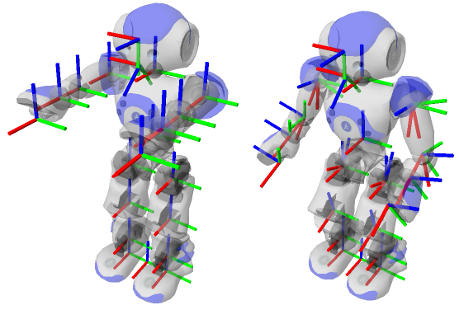
\includegraphics[width=0.8\textwidth]{Images/background_and_tools/tf_tree.png}
	\caption{\textit{A robot in 2 different positions, with} tf \textit{frames in evidence: x-axis is red, y-axis is green, z-axis is blue. The frames are the same in both configuration, but the transformations (i.e. rototranslations) between them are different}}
	\label{fig:tfTreeRviz}
\end{figure}

\begin{figure}
	\centering
	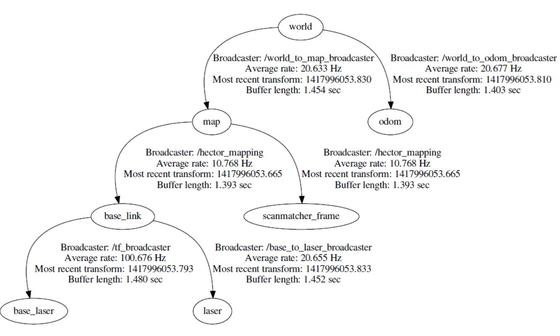
\includegraphics[width=0.6\textwidth]{Images/background_and_tools/tfGraph.JPG}
	\caption{\textit{An example of} tf \textit{tree}}
	\label{fig:tfGraph}
\end{figure}

In figure \ref{fig:tfTreeRviz} you can see a graphical representation of the reference frames tracked in a Nao Robot, while figure \ref{fig:tfGraph} shows an example of \textit{tf} graph visualizad with a the visualization framework \textit{rqt}. 


\section{Odometry}\label{sec:odometry}
Odometry is a very important 
\begin{itemize}
	\item cosa si intende per odometria
	\item motion models: differential drive e skid steering
	\item sensor fusion cos'è, e esempio di Robot localization
	\item localizzazione con amcl
\end{itemize}

\section{Navigation Stack}\label{sec:navigationStack}
SKETCH:
\begin{itemize}
	\item cos'è navigation stack (immagine http://wiki.ros.org/move\_base?action=AttachFile\&do=get\&target=overview\_tf.png)
	\item local/global costmap
\end{itemize}